%!TEX builder = latexmk
%!TEX program = pdflatex
%!TEX option = -shell-escape
\documentclass[oneside,english]{book}

\usepackage[T1]{fontenc}
\usepackage[normalem]{ulem}
\usepackage[letterpaper]{geometry}
\geometry{verbose,tmargin=1in,bmargin=1in,lmargin=1in,rmargin=1in}

% table of contents and numbering
\usepackage{tocbibind}
%\setcounter{secnumdepth}{3}
\setcounter{tocdepth}{3}
\usepackage{babel}
\usepackage{float}
\usepackage{textcomp}
\usepackage{amsfonts,amsmath,amssymb,mathptmx}
\usepackage{mathrsfs}
\usepackage[colorlinks, citecolor=blue, linkcolor=black, anchorcolor=black]{hyperref}
%code
\usepackage{listings}
% colors to show the corrections
\usepackage[dvipsnames,usenames]{xcolor}
\definecolor{light-gray}{rgb}{0.7,0.7,0.7}
\definecolor{dark-gray}{rgb}{0.1,0.1,0.3}
\definecolor{light-blue}{rgb}{0.7,0.7,0.9}
\definecolor{dark-blue}{rgb}{0.2,0.2,0.5}

\colorlet{punct}{red!60!black}
\definecolor{background}{HTML}{EEEEEE}
\definecolor{delim}{RGB}{20,105,176}
\colorlet{numb}{magenta!60!black}

\lstdefinelanguage{json}{
    basicstyle=\normalfont\ttfamily,
    %numbers=left,
    %numberstyle=\scriptsize,
    %stepnumber=1,
    %numbersep=8pt,
    showstringspaces=false,
    breaklines=true,
    frame=lines,
    backgroundcolor=\color{background},
    literate=
     *{0}{{{\color{numb}0}}}{1}
      {1}{{{\color{numb}1}}}{1}
      {2}{{{\color{numb}2}}}{1}
      {3}{{{\color{numb}3}}}{1}
      {4}{{{\color{numb}4}}}{1}
      {5}{{{\color{numb}5}}}{1}
      {6}{{{\color{numb}6}}}{1}
      {7}{{{\color{numb}7}}}{1}
      {8}{{{\color{numb}8}}}{1}
      {9}{{{\color{numb}9}}}{1}
      {:}{{{\color{punct}{:}}}}{1}
      {,}{{{\color{punct}{,}}}}{1}
      {\{}{{{\color{delim}{\{}}}}{1}
      {\}}{{{\color{delim}{\}}}}}{1}
      {[}{{{\color{delim}{[}}}}{1}
      {]}{{{\color{delim}{]}}}}{1},
}
\lstset{
    language=C,
    columns=fixed,       
    frame=no, %tb,                                     
    %backgroundcolor=\color[RGB]{244,244,244},            
    keywordstyle=\color[RGB]{40,40,255},                 
    %numberstyle=\footnotesize\color{darkgray},           
    commentstyle=\it\color[RGB]{0,96,96},                
    stringstyle=\rmfamily\slshape\color[RGB]{128,0,0},   
    showstringspaces=false,                                                          
    basicstyle=\small\ttfamily, %\scriptsize%\tiny%\footnotesize  
    breaklines=true
}


\IfFileExists{url.sty}{\usepackage{url}}
                      {\newcommand{\url}{\texttt}}

% biblio
\usepackage[authoryear]{natbib}
% biblio GJI
\bibliographystyle{abbrvnat}

% fonts
\usepackage{times}

% figures
\usepackage{graphicx}

% we are running pdflatex, so convert .eps files to .pdf
%\usepackage[dvips]{epsfig}
\usepackage{enumitem}
\setitemize[1, 2]{topsep=0em, itemsep=0.0em, partopsep=0em, leftmargin=1em}

\usepackage{fancyhdr}
%\usepackage{breakurl}

% BibTeX logo
\newcommand{\BibTeX}{{\rm B\kern-.05em{\sc i\kern-.025em b}\kern-.08em{T}\kern-.1667em\lower.7ex\hbox{E}\kern-.125emX}}

\graphicspath{{./figure}}

\setlength{\parskip}{0.4em}

%%%%%%%%%%%%%%%%%%%%%%%%%%%%%% Start of document.

\begin{document}


%%%%%%%%%%%%%%%%%%%%%%%%%%%%%%%%%%%%%%%%%%%%%%%%%
%% TITLE page
%%%%%%%%%%%%%%%%%%%%%%%%%%%%%%%%%%%%%%%%%%%%%%%%%
%\begin{center}
%\thispagestyle{empty}\vspace*{-1.8truecm} %
%\makebox[1\textwidth]{%
%\includegraphics[width=0.83\paperwidth]{figures/.pdf} %
%}
%\par\end{center}


\title{\textbf{CGFD2D-wave}\\
       \textbf{User Manual}}


\author{\copyright \, zwlab}

% date of last edit
\date{\today}

\maketitle

%%%%%%%%%%%%%%%%%%%%%%%%%%%%%%%%%%%%%%%%%%%%%%%%%

\newpage{}


%%%%%%%%%%%%%%%%%%%%%%%%%%%%%%%%%%%%%%%%%%%%%%%%%
%% Table of contents
%%%%%%%%%%%%%%%%%%%%%%%%%%%%%%%%%%%%%%%%%%%%%%%%%

\newpage

\tableofcontents

%%%%%%%%%%%%%%%%%%%%%%%%%%%%%%%%%%%%%%%%%%%%%%%%%

%\include{01_introduction}

\chapter{How to give media parameters and run wave simulations for different media types}\label{chapter-media}

\markright{CHAPTER \ref{chapter-media} MEDIA}
%\markrright{Media}
\begin{lstlisting}[language=json, title=par.json, frame=tb]
  "medium" : {
      "type"  : "elastic_aniso",
      "#code_generate" : 1,
      "infile_layer" : "/home/usr1/testCGFD2D/prep_medium/basin.mdlay",
      "#infile_grid" : "/home/usr1/testCGFD2D/prep_medium/basin.mdgrd",
      "#import" : "/home/usr1/testCGFD2D/output/media",
      "equivalent_medium_method" : "tti"
  },
  "is_export_media" : 1,
  "media_export_dir" : "/home/usr1/testCGFD2D/output/media",

  "#visco_config" : {
      "type" : "graves_Qs",
      "Qs_freq" : 1.0
  } 
\end{lstlisting}

\begin{itemize}
  % TODO: waveform eqn. should be given and analyzed before
  \item \texttt{type} is the flag of the solver, that is, what media do you want to simulate, and four options are supported in this code:
  \begin{itemize}
    \item \texttt{acoustic\_iso}: choose this to call the solver of acoustic wave equation of isotropic media.  
    \item \texttt{elastic\_iso}: choose this to call the solver of the elastic wave equation of isotropic media.
    \item \texttt{elastic\_vti}: choose this to call the solver of the elastic wave equation of vertical transversely isotropic media. 
    \item \texttt{elastic\_aniso}: choose this to call the solver of the elastic wave equation of anisotropic media. 
  \end{itemize}
  The media type is given in \texttt{import}, \texttt{code\_generate}, \texttt{infile\_layer} or \texttt{infile\_grid}.
  
  \item The media can be given in four ways:
  \begin{itemize}  
    \item \texttt{code\_generate}: Choose this flag if you want to give the media by code. You should edit \textbf{forward/md\_t.c} file and recompile the code.
    \item \texttt{infile\_layer}: If you want to give media by the intereface line, this option should be helpful. The media parameters are given by the \textbf{mdlay} file, and the file format is shown in Section \ref{mdlay} 
    \item \texttt{infile\_grid}: If you want to give media by a given grid media, this option should be helpful. The media parameters are given by the \textbf{mdgrd} file, the file format is shown in Section \ref{mdgrd}.
    \item \texttt{import}: If you already generated media from the above three options, and do not want to re-generate media, select this option and give the folder of the exported media. 
  \end{itemize}
  
  \item \texttt{equivalent\_medium\_method}: If you give media by \texttt{infile\_layer} or \texttt{infile\_grid}, equivalent medium parameterization methods can be applied. For different media, we provide different equivalent medium parameterization methods, please see Section \ref{equivalent_method} for detail.
  
  \item \texttt{is\_export\_media} should be \textbf{1} if you want to export the media, and a \textbf{media\_export\_dir} should be given. 
  
  \item The \texttt{visco\_config} is selected if the media is viscoelastic, the visco\_type and Qs frequency are needed.

\end{itemize}


%===================================================================
\section{Format of .mdlay} \label{mdlay}

If you want to get the model from the interface line, you can select the option \texttt{infile\_layer}.
And the media are given by a \textbf{mdlay} file. The file format is:
\begin{itemize}
 \item The first line is the media type, it can be \\
 \texttt{one\_component}, \\ 
 \texttt{acoustic\_isotropic}, \\
 \texttt{elastic\_isotropic}, \\
 \texttt{elastic\_vti\_prem}, \\
 \texttt{elastic\_vti\_thomsen}, \\ 
 \texttt{elastic\_vti\_cij}, \\
 \texttt{elastic\_tti\_thomsen}, \\ 
 \texttt{elastic\_tti\_bond}, \\
 \texttt{elastic\_aniso\_cij}.

 \item The second line is the number of interface (\texttt{NI}).

 \item After then, for each interface below, give the number of points (\texttt{npoints}) and then x, z, and media parameters for each point. Take the \texttt{elastic\_isotropic} media for example, the media parameters are read as:
 \begin{lstlisting}[language=C]
  for (ni=0; ni<NI; ni++) 
    for (ip=0; ip<npoints; ip++) 
        fscanf(layer_file, "%f %f %f %f %f %f %f %f %f %f %f", 
               &x_interface, &z_interface,
               &rho, &rho_grad, &rho_pow,
               &vp, &vp_grad, &vp_pow,
               &vs, &vs_grad, &vs_pow);
 \end{lstlisting}
 Note that the \texttt{x} here need to be increasing, the max range of interfaces need to be lager than the calculation area in x direction. 
 \texttt{*\_grad} and \texttt{*\_pow} is the gradient and power of the media parameters in z-direction. The media parameters below interface are calculated by
 \begin{equation*}
    var_{grid~point} = var + \left( z\text{\_interface}-z_{grid~point} \right)^{var\_pow} * var\_grad.
 \end{equation*}
For the points higher than the interface, assigned by the uppermost medium. The media parameters in x-direction are calculated by linear interpolation.

For different media type, different media parameters are given,
\begin{itemize}
  \item \texttt{one\_component}: var, var\_grad, var\_pow.

  \item \texttt{acoustic\_isotropic}: $\rho$, $\rho\_grad$, $\rho\_pow$, $vp$, $vp\_grad$, $vp\_pow$.

  \item \texttt{elastic\_isotropic}: $\rho$, $\rho\_grad$, $\rho\_pow$, vp, vp\_grad, vp\_pow, vs, vs\_grad, vs\_pow.

  \item \texttt{elastic\_vti\_prem}: $\rho$, $\rho\_grad$, $\rho\_pow$, vph, vph\_grad, vph\_pow, vpv, vpv\_grad, vpv\_pow, vsv, vsv\_grad, vsv\_pow, $\eta$, $\eta$\_grad, $\eta$\_pow. The meaning of the media parameters can be found from \citep{dziewonski1981preliminary}.

  \item \texttt{elastic\_vti\_thomsen}: $\rho$, $\rho\_grad$, $\rho\_pow$, $\alpha_0$, $\alpha_0$\_grad, $\alpha_0$\_pow, $\beta_0$, $\beta_0$\_grad, $\beta_0$\_pow, $\epsilon$, $\epsilon$\_grad, $\epsilon$\_pow, $\delta$, $\delta$\_grad, $\delta$\_pow. The meaning of the media parameters can be found from \citep{thomsen1986weak}.
  
  \item \texttt{elastic\_vti\_cij}: $\rho$, $\rho\_grad$, $\rho\_pow$, $c_{11}$, $c_{11}\_grad$, $c_{11}\_pow$, $c_{33}$, $c_{33}\_grad$, $c_{33}\_pow$, $c_{55}$, $c_{55}\_grad$, $c_{55}\_pow$, $c_{13}$, $c_{13}\_grad$, $c_{13}\_pow$. 

  \item \texttt{elastic\_tti\_thomsen}: $\rho$, $\rho\_grad$, $\rho\_pow$, $\alpha_0$, $\alpha_0\_grad$, $\alpha_0\_pow$, $\beta_0$, $\beta_0\_grad$, $\beta_0\_pow$, $\epsilon$, $\epsilon\_grad$, $\epsilon\_pow$, $\delta$, $\delta\_grad$, $\delta\_pow$, $\theta$, $\theta\_grad$, $\theta\_pow$. The meaning of the media parameters can be found from \citep{thomsen1986weak}.

  \item \texttt{elastic\_tti\_bond}: $\rho$, $\rho\_grad$, $\rho\_pow$, $c_{11}$, $c_{11}\_grad$, $c_{11}\_pow$, $c_{33}$, $c_{33}\_grad$, $c_{33}\_pow$, $c_{55}$, $c_{55}\_grad$, $c_{55}\_pow$, $c_{13}$, $c_{13}\_grad$, $c_{13}\_pow$, $\theta$, $\theta\_grad$, $\theta\_pow$. $\theta$ is the dip angle.

  \item \texttt{elastic\_aniso\_cij}: $\rho$, $\rho\_grad$, $\rho\_pow$, $c_{11}$, $c_{11}\_grad$, $c_{11}\_pow$, $c_{13}$, $c_{13}\_grad$, $c_{13}\_pow$, $c_{15}$, $c_{15}\_grad$, $c_{15}\_pow$, $c_{33}$, $c_{33}\_grad$, $c_{33}\_pow$, $c_{35}$, $c_{35}\_grad$, $c_{35}\_pow$, $c_{55}$, $c_{55}\_grad$, $c_{55}\_pow$.
\end{itemize}

\end{itemize}
You can also find examples in the \textbf{example/prep\_medium} directory.

%=============================================================
\section{Format of .mdgrd} \label{mdgrd}

The option \texttt{infile\_grid} is useful if you want to give the media by a grid model.
If \texttt{infile\_grid} is selected, the media should be given by a \textbf{.mdgrd} file. The file format is:
\begin{itemize}
 \item The first line is the media type, it can be \\
 \texttt{one\_component}, \\ 
 \texttt{acoustic\_isotropic}, \\
 \texttt{elastic\_isotropic}, \\
 \texttt{elastic\_vti\_prem}, \\
 \texttt{elastic\_vti\_thomsen}, \\ 
 \texttt{elastic\_vti\_cij}, \\
 \texttt{elastic\_tti\_thomsen}, \\ 
 \texttt{elastic\_tti\_bond}, \\
 \texttt{elastic\_aniso\_cij}.

 \item The second line is the number of layer (\texttt{NL}), if \texttt{NL} > 1, there is a designated interface, and the equivalent medium parameterization methods can be applied across this interfaces.

 \item The next \texttt{NL} lines are the number of grids in the z-direction of each layer 

 \item {Next, the information of the interface mesh is given:\\
  \texttt{NX} ~~ \texttt{MIN\_X}  ~~ \texttt{SPACING\_X}\\
  \texttt{NX} is the number of points along $x$ direction; \\
  \texttt{MIN\_X} is the minimal $x$ coordinates; \\
  \texttt{SPACING\_X} is spacing between points along $x$.
 }

 \item {
  After then, the elevation, media parameters are given in every grid points. Take the \texttt{elastic\_isotropic} media for example, the media parameters are read as:
  \begin{lstlisting}[language = C]
  for (nl=0; nl< NL; nl++)
    for (ip=0; ip<np[nl]; np++)
      for (ix=0; ix<NX; ix++)  
        fscanf(in_file_grid, "%f %f %f %f", 
              &elevation, &rho, &vp, &vs);
  \end{lstlisting}
 } 

The media parameters are calculated by interpolation of the values at the given grid points.

For the points higher than the interface, assigned by the uppermost medium. 

For different media type, different media parameters are given,
\begin{itemize}
  \item \texttt{one\_component}: var.

  \item \texttt{acoustic\_isotropic}: $\rho$, vp.

  \item \texttt{elastic\_isotropic}: $\rho$, vp, vs.

  \item \texttt{elastic\_vti\_prem}: $\rho$, vph, vpv, vsv, $\eta$. Please see \citep{dziewonski1981preliminary} for detail.

  \item \texttt{elastic\_vti\_thomsen}: $\rho$, $\alpha_0$, $\beta_0$, $\epsilon$, $\delta$. Please see \citep{thomsen1986weak} for detail.

  \item \texttt{elastic\_vti\_cij}: $\rho$, $c_{11}$, $c_{33}$, $c_{55}$, $c_{13}$. 

  \item \texttt{elastic\_tti\_thomsen}: $\rho$, $\alpha_0$, $\beta_0$, $\epsilon$, $\delta$, $\theta$. Please see \citep{thomsen1986weak} for detail.

  \item \texttt{elastic\_tti\_bond}: $\rho$, $c_{11}$, $c_{33}$, $c_{55}$, $c_{13}$, $\theta$. $\theta$ is the dip angle.

  \item \texttt{elastic\_aniso\_cij}: $\rho$, $c_{11}$, $c_{13}$, $c_{15}$, $c_{33}$, $c_{35}$, $c_{55}$.
\end{itemize}

\end{itemize}

If \texttt{NL} > 1, there is a designated interface; and the elevation of ng[il]+1 needs to be the same as ng[il]. The equivalent medium parameterization method can be applied on the points cutting by this interface.

You can also find the example in the \textbf{example/prep\_medium} directory.

%===================== equivalent medium para method ===========================
\section{Note about equivalent medium parameterization methods} \label{equivalent_method} 
When there are strong interfaces in the model, using grid points to discrete models directly may cause interface error and the generation of artificial diffraction from stair step interfaces. In this code, we provide some equivalent medium parametrization methods to reduce this interface error.

If you give the model by \texttt{infile\_layer} or \texttt{infile\_grid}, you can apply different equivalent medium parametrization methods by give different \texttt{equivalent\_medium\_method}. 

\begin{figure}[H]
\centering 
  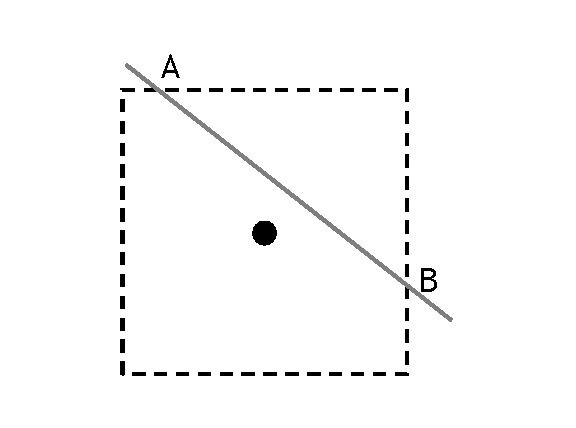
\includegraphics[width=0.3\linewidth]{figure/grid_inclined.pdf}
  \caption{Illustration of an interface passing through an FD cell. The black circle represents the grid point, the dashed-line square represents a finite0-difference mesh centred on the black circle. The equivalent medium parameterization methods are act on such grid points passed through by the interfaces.}
  \label{equi_grid}
\end{figure}

If the media type in the \textbf{mdgrd} or \textbf{mdlay} file is \texttt{one\_component}, \texttt{equivalent\_medium\_method} can be
\begin{itemize}
 \item \texttt{loc}: using local value to discrete model. 
 \item \texttt{ari}: volume integral arithmetic average, 
  \begin{align}
    \left<var\right> = \frac{1}{\Delta V} \int_{iz-1/2}^{iz+1/2} \int_{ix-1/2}^{ix+1/2} var~dx dz
  \end{align}
 \item \texttt{har}: volume integral harmonic average. 
  \begin{align}
    \left<var\right>^H = \frac{\Delta V}{\int_{iz-1/2}^{iz+1/2} \int_{ix-1/2}^{ix+1/2} \frac{1}{var} dx dz}
  \end{align}
\end{itemize}

If the media type is \texttt{acoustic\_isotropic}, \texttt{equivalent\_medium\_method} can be
\begin{itemize}
 \item \texttt{loc}: using local media parameters to discrete model. 
 \item \texttt{har}: applying harmonic average to $\kappa$, and applying arithmetic average to density $\rho$. 
 \item \texttt{ari}: applying arithmetic average to $\kappa$ and $\rho$. 
\end{itemize}

If the media type is \texttt{elastic\_isotropic}, \texttt{equivalent\_medium\_method} can be
\begin{itemize}
 \item \texttt{loc}: using local media parameters to discrete model. 
 \item \texttt{har}: applying harmonic average to elastic modulus, and applying arithmetic average to density $\rho$. See \citet{moczo_3d_2002} and \citep{moczo_finite-difference_2014} for detail.
 \item \texttt{ari}: applying arithmetic average to elastic modulus and density. 
 \item \texttt{tti}: applying TTI representation to elastic modulus and arithmetic average to density. See \citep{jiang2021tti} for detail. 
\end{itemize}

If the media type is \texttt{elastic\_vti\_*}, \texttt{equivalent\_medium\_method} can be
\begin{itemize}
 \item \texttt{loc}: using local media parameters to discrete model. 
 \item \texttt{har}: applying harmonic average to elastic modulus $c_{ij}$, and applying arithmetic average to density $\rho$.
 \item \texttt{ari}: applying arithmetic average to elastic modulus $c_{ij}$ and density. 
 \item \texttt{tti}: applying TTI representation to elastic modulus and arithmetic average to density.
\end{itemize}

If the media type is \texttt{elastic\_aniso\_cij} or \texttt{elastic\_tti\_*}, \texttt{equivalent\_medium\_method} can be
\begin{itemize}
 \item \texttt{loc}: using local media parameters to discrete model. 
 \item \texttt{har}: applying harmonic average to elastic modulus $c_{ij}$, and applying arithmetic average to density $\rho$.
 \item \texttt{ari}: applying arithmetic average to elastic modulus $c_{ij}$ and density. 
\end{itemize}


\chapter*{Copyright}
\addcontentsline{toc}{chapter}{Copyright}

Main historical authors: \\

$\copyright$ October 2021\\

\noindent
This program is free software; you can redistribute it and/or modify
it under the terms of the xxx License as published 
by the Free Software Foundation (see xxx).\\

\noindent
Please note that by contributing to this code, the developer understands and agrees that this project and contribution
are public and fall under the open source license mentioned above.\\

\noindent
\textbf{\underline{Evolution of the code:}}\\


%%%%%%%%%%%%%%%%%%%%%%%%%%%%%%%%%%%%%%%%%%%%%%%%%
%% REFERENCES
%%%%%%%%%%%%%%%%%%%%%%%%%%%%%%%%%%%%%%%%%%%%%%%%%
%in every chapter
\bibliography{citation}

%%%%%%%%%%%%%%%%%%%%%%%%%%%%%%%%%%%%%%%%%%%%%%%%%
%% APPENDIX
%%%%%%%%%%%%%%%%%%%%%%%%%%%%%%%%%%%%%%%%%%%%%%%%%

\appendix

%\include{A_reference_frame}

%%%%%%%%%%%%%%%%%%%%%%%%%%%%%%%%%%%%%%%%%%%

\end{document}
